% Metódy inžinierskej práce

% Na úkor 4teho cvicenia
\documentclass[10pt,twocolumn,twoside,slovak,a4paper]{article}
%\documentclass[10pt,twoside,slovak,a4paper]{article}

\usepackage[slovak,english]{babel}
%\usepackage[T1]{fontenc}
\usepackage[IL2]{fontenc} % lepšia sadzba písmena Ľ než v T1
\usepackage[utf8]{inputenc}
\usepackage{graphicx}
\usepackage{url} % príkaz \url na formátovanie URL
\usepackage{hyperref} % odkazy v texte budú aktívne (pri niektorých triedach dokumentov spôsobuje posun textu)
\usepackage{wrapfig}

\usepackage{cite}
%\usepackage{times}

\pagestyle{headings}

\title{Spotify recommendation system and its flaws\thanks{Semestrálny projekt v predmete Metódy inžinierskej práce, ak. rok 2024/25, vedenie: Mgr. Yevheniia Kataieva, PhD.}} % meno a priezvisko vyučujúceho na cvičeniach

\author{Timon Lumír Fillo\\[2pt]
	{\small Slovenská technická univerzita v Bratislave}\\
	{\small Fakulta informatiky a informačných technológií}\\
	{\small \texttt{xfillo@stuba.sk}}
	}

\date{\small \today} % upravte

\selectlanguage{english}
\begin{document}

\maketitle

\begin{abstract}

The digitalization of music has brought about a great change to the way we perceive and experience music, with companies such as Spotify, YouTube Music and Apple Music that offer online music streaming of millions of tracks for anyone that has access to the internet. This has made globalization of music possible and enabled artists to reach their target audience on the other side of the globe, which has in turn opened up new music markets all around the world and enabled even small artists to make a living from music production. All of this would not be possible without a recommendation system that can accurately
\begin{wrapfigure}{r}{0.5\textwidth}
\centering

\includegraphics[width=0.3\textwidth]{fiitLogo/PNG/STU-FIIT-nfnh.png}
\end{wrapfigure} 
categorize and find music that will satisfy the listener. While these systems provide relevant music recommendations, they come at the cost of indirectly altering the creative process of creators and limit creativity at the expense of generating income. This factor is mostly prevalent in trending music that is made specifically to exploit the recommendation system's inner workings with the aim of targeting a wider audience, earning revenue, and receiving more streams. This paper will explore what algorithms make up Spotify's recommendation system, how these algorithms affect the listeners, and how they affect the artists and record labels.

\end{abstract}



\section{Introduction}
Test na citáciu
\cite{hodgson2021spotify}
\dots

\section{Cvičenie 4}
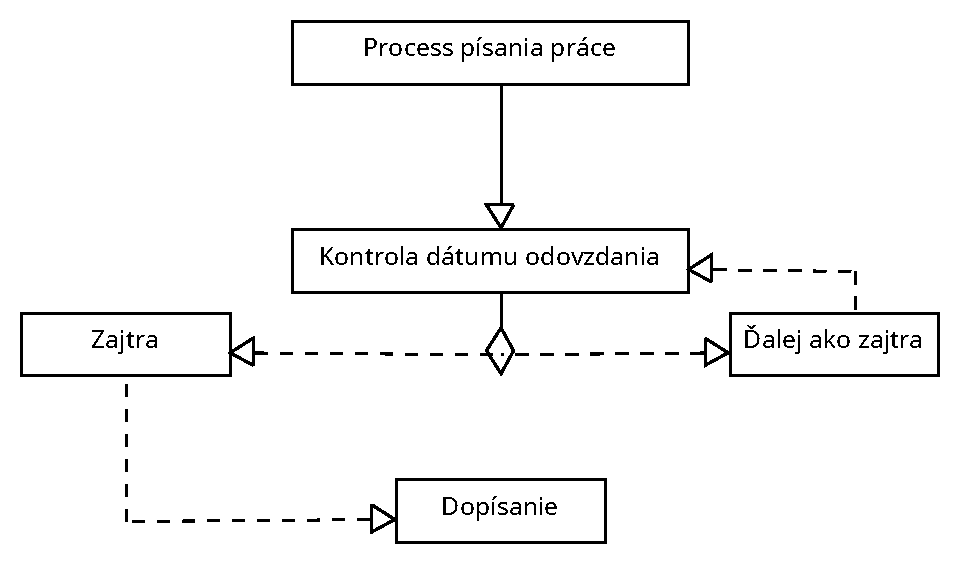
\includegraphics[width=0.5\linewidth]{graphics/diagram1.pdf}
\hfil
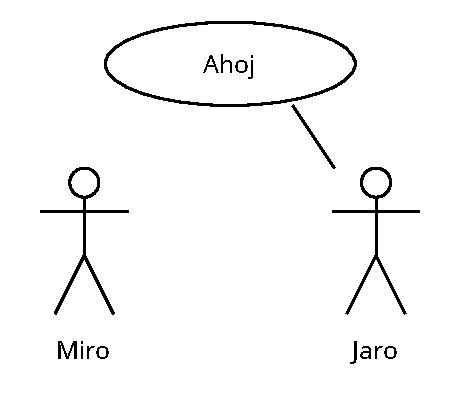
\includegraphics[width=0.5\linewidth,angle=45]{graphics/kamosi.pdf}

\begin{tabular}{|c|c|c|c|c|}
\hline
	1&2&3&4&5\\
\hline
	6&7&8&9&10\\
\hline
	11&12&13&14&15\\
\hline
	16&17&18&19&20 \\
\hline
\end{tabular}

\begin{equation}
	1+2+3+4+5+6+7+8+9+10+11+12+13+14+15+16+17+18+19+20=210
\end{equation}
% Pointa je ukázať ako spotify recommendation system funguje a ako jeho fungovanie ovplyvnuje celý hudboný industry
% Vplyv trendov na recommendation systémy a spätne
% Kritika že recommendation system preferuje krátke a vysoko emočne zafarbené skladby čím sa z trhu vytláčajú vážnejšie žánre, ktoré majú dlhšie skladby a niesú nositeľmi silného affektu
\section{Spotify}\label{spotify}
% Čo je spotify, čo ponúka, aký ma vplyv na hudbu a víziu
\dots

\section{Recommendation system}\label{recommendationsystem}
% Ako funguje, na akých dátach vyhodnocuje odporúčanie
% Ako sa spotify vypláca artistov a ako to ovplyvňuje recommendation system
\dots

\section{Genre representation}\label{genre}
% Ktoré žánre profitujú z tohto recommendation systému a ktoré zase nie
% Nové žánre alebo adaptácia už existujúcich ako dôsledok recommendation systemu
\dots

\section{Conclusion}\label{conclusion} % prípadne iný variant názvu
% Návrh na zlepšenie a zbavenie sa problémov
\dots

%\acknowledgement{Ak niekomu chcete poďakovať\ldots}


% týmto sa generuje zoznam literatúry z obsahu súboru literatura.bib podľa toho, na čo sa v článku odkazujete
%\newpage
%\listoftodos[Notes]
\bibliographystyle{abbrv} % prípadne alpha, abbrv alebo hociktorý iný
\bibliography{literatura}

\end{document}
